\documentclass[10pt,twocolumn]{article}

\usepackage[margin=0.75in]{geometry}
\usepackage{array}
\usepackage{booktabs}
\usepackage{hyperref}
\usepackage{tikz}
\usepackage{url}
\usetikzlibrary{arrows.meta,positioning}

\title{Diagnosing Hybrid Attention/Mamba Cache Over-Reservation from vLLM Planner Artifacts}
\author{Anonymous Workshop Submission}
\date{}

\newcommand{\tool}{Cachepawl}
\newcommand{\pathc}{Path C}
\newcommand{\plannerpad}{uniform padded}
\newcommand{\plannernative}{native KV/state}

\begin{document}

\maketitle

\begin{abstract}
Hybrid Attention/Mamba language models put heterogeneous cache state behind a
serving interface designed largely around uniform KV pages. This mismatch can
cause a planner to reserve more memory than the useful hybrid cache payload,
but measuring the gap is difficult without first separating planner evidence
from runtime mutation. We present \tool{} \pathc, a read-only workflow that
captures vanilla vLLM cache-plan artifacts, translates them into an advisory
schema, replays the planner stage on captured inputs, and reports
planner-level over-reservation. In a bounded four-cell matrix for
\texttt{Zyphra/Zamba2-2.7B-instruct} under \texttt{vllm==0.21.0}, the observed
planner artifacts show advisory savings from 0.64 to 1.26 GiB
(685,011,456 to 1,347,563,520 bytes), with overestimation ratio
1.7333734577189286. A separate deterministic RTX 3060 planner-only pack shows
that a native KV/state planner model stays within 1.007x of useful bytes on
three synthetic hybrid workloads, while a uniform padded planner model ranges
from 2.869x to 3.934x. These are planner/advisory results, not runtime cache
substitution or serving-performance measurements.
\end{abstract}

\section{Introduction}

Serving systems increasingly need to plan memory for models whose internal
state is not uniform. Transformer-serving systems popularized page-based KV
cache management because each attention layer grows with the sequence and can
be handled through a common block abstraction. Hybrid Attention/Mamba models
break that simplifying assumption. Attention layers still consume KV pages,
but Mamba or SSM layers carry state tensors with a different shape and reuse
contract. If a serving planner accounts for both through one padded page shape,
reserved memory can diverge from useful cache payload.

The systems question is not only whether a better allocator might exist. Before
runtime integration is meaningful, we need to know whether the planner inputs
and cache artifacts already expose the mismatch. A diagnostic workflow should
answer three narrower questions. First, can a vanilla serving run be observed
without mutating scheduler, allocator, or worker state? Second, can the cache
plan be translated into a stable schema that separates useful bytes from
reserved bytes? Third, does planner replay agree with the runtime scheduler
configuration closely enough to support an advisory comparison?

This paper answers those questions for a bounded vLLM \pathc{} evidence pack.
The result is intentionally narrower than a serving-system replacement. It is
a workshop-scale diagnostic study of planner artifacts for hybrid cache
layouts, with an explicit boundary between advisory evidence and future
controlled substitution. That boundary makes the contribution more useful, not
less: it identifies what can be concluded from committed artifacts today and
what must be measured before stronger runtime claims are appropriate.

\textbf{Contributions.}
This paper makes four contributions:

\begin{itemize}
\item an observe/translate/replay/diagnose workflow for read-only analysis of
vLLM hybrid cache-plan artifacts;
\item a bounded \pathc{} matrix showing planner-level over-reservation for one
\texttt{Zyphra/Zamba2-2.7B-instruct} setup;
\item a deterministic RTX 3060 planner-only comparison showing the gap between
a \plannerpad{} planner model and a \plannernative{} planner model;
\item a compact artifact and claim boundary that keeps runtime substitution,
serving memory savings, latency, throughput, and quality in future work.
\end{itemize}

\section{Background and Related Work}

\textbf{Paged serving systems.}
PagedAttention and vLLM introduced a virtualized KV-cache view that lets
serving systems manage transformer KV memory efficiently at request granularity
\cite{kwon2023pagedattention}. SGLang targets efficient execution of structured
language model programs and provides another planner-facing serving context
\cite{zheng2024sglang}. This paper uses the same systems lens: cache planning
is a concrete runtime decision, and planner artifacts can be studied directly.

\textbf{Hybrid architectures.}
Jamba and Zamba2 combine attention with Mamba-style sequence modeling
\cite{lieber2024jamba,glorioso2024zamba2}. These models motivate heterogeneous
cache accounting because attention KV pages and Mamba state tensors do not
share a single natural memory shape. The issue is not simply larger models; it
is mixed state with different byte geometry.

\textbf{Diagnostics before substitution.}
The closest framing for this paper is artifact-based systems diagnosis. Rather
than replacing a runtime allocator, \tool{} \pathc{} asks what can be inferred
from a captured planner state. This is a lower-risk step toward integration:
planner diagnostics can show over-reservation in an observed plan, but they do
not establish live VRAM reduction, request-admission improvement, latency,
throughput, or model quality.

\section{Method}

\begin{figure*}[t]
\centering
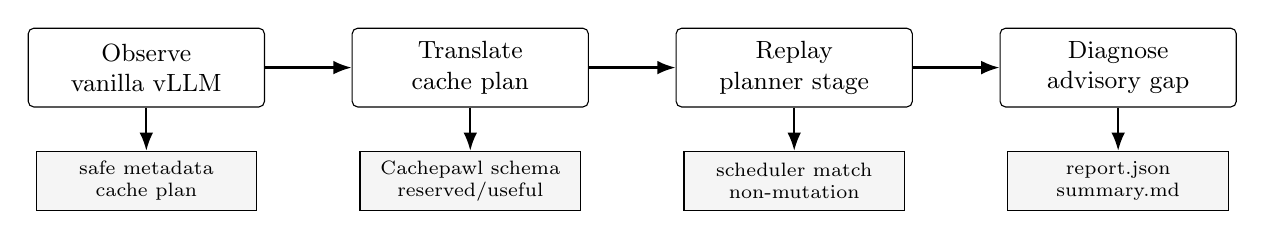
\begin{tikzpicture}[
  node distance=1.1cm,
  stage/.style={draw, rounded corners=2pt, align=center, minimum width=3.0cm,
    minimum height=1.0cm, font=\small},
  artifact/.style={draw, align=center, minimum width=2.8cm, minimum height=0.75cm,
    font=\scriptsize, fill=gray!8},
  arrow/.style={-Latex, thick}
]
\node[stage] (observe) {Observe\\vanilla vLLM};
\node[stage, right=of observe] (translate) {Translate\\cache plan};
\node[stage, right=of translate] (replay) {Replay\\planner stage};
\node[stage, right=of replay] (diagnose) {Diagnose\\advisory gap};

\node[artifact, below=0.55cm of observe] (raw) {safe metadata\\cache plan};
\node[artifact, below=0.55cm of translate] (schema) {\tool{} schema\\reserved/useful};
\node[artifact, below=0.55cm of replay] (match) {scheduler match\\non-mutation};
\node[artifact, below=0.55cm of diagnose] (report) {report.json\\summary.md};

\draw[arrow] (observe) -- (translate);
\draw[arrow] (translate) -- (replay);
\draw[arrow] (replay) -- (diagnose);
\draw[arrow] (observe) -- (raw);
\draw[arrow] (translate) -- (schema);
\draw[arrow] (replay) -- (match);
\draw[arrow] (diagnose) -- (report);
\end{tikzpicture}
\caption{Read-only \pathc{} workflow. The workflow converts captured vLLM
planner artifacts into advisory metrics without returning a \tool{} plan to
the serving runtime.}
\label{fig:workflow}
\end{figure*}

Figure~\ref{fig:workflow} shows the \pathc{} workflow. The design principle is
that all measurements come from artifacts and replay, not mutation.

\subsection{Observe}

The observed run uses \texttt{Zyphra/Zamba2-2.7B-instruct} with
\texttt{vllm==0.21.0}. The observation phase records the runtime cache plan,
planner metadata, scheduler and KV-manager structure, worker tensor layout,
request-to-block assignment, and attention block-table metadata. It does not
edit vLLM source, monkeypatch runtime methods, replace allocators, or return
\tool{} plans to vLLM.

\subsection{Translate and Replay}

The translation step maps the observed cache plan into fields needed for
advisory accounting: cache group count, cache tensor count, layer count, block
count, per-group cache kind, page size, block size, useful bytes, and observed
reserved bytes. The replay step reruns vLLM's planner configuration routine on
captured planner inputs. In the committed evidence, replay matches the runtime
scheduler cache configuration and records that runtime state did not change
during replay.

\subsection{Diagnose}

The diagnostic report computes five planner-level quantities:
reserved bytes, useful bytes, advisory savings bytes, overestimation ratio, and
wasted fraction. For a plan with reserved bytes $R$ and useful bytes $U$, the
reported ratio is $R/U$, and the wasted fraction is $(R-U)/R$. These metrics
are deliberately planner-facing. They quantify over-reservation in the
observed or modeled planner state.

\section{Evaluation}

The evaluation has two tracks. The first uses observed vLLM planner artifacts
for a bounded matrix over one hybrid model. The second uses a deterministic
planner-only comparison over synthetic hybrid workloads for an RTX 3060 target
profile. Both tracks measure planner estimates.

\subsection{Observed vLLM Planner Matrix}

Table~\ref{tab:pathc} reports the four completed \pathc{} cells. Values are
shown in GiB to keep the table readable; exact byte values appear in the
supplement and committed matrix artifact.

\begin{table}[t]
\centering
\small
\begin{tabular}{ccccc}
\toprule
Len & Util. & Reserved & Useful & Savings \\
 & & GiB & GiB & GiB \\
\midrule
2048 & 0.6 & 1.76 & 1.02 & 0.75 \\
2048 & 0.7 & 2.97 & 1.71 & 1.26 \\
4096 & 0.6 & 1.51 & 0.87 & 0.64 \\
4096 & 0.7 & 2.71 & 1.56 & 1.15 \\
\bottomrule
\end{tabular}
\caption{\pathc{} advisory matrix for
\texttt{Zyphra/Zamba2-2.7B-instruct}. Across these cells the overestimation
ratio is 1.7333734577189286 and the wasted fraction is 0.4230902777777778.}
\label{tab:pathc}
\end{table}

\textbf{Interpretation.}
The observed planner artifacts reserve substantially more than the useful
hybrid cache payload in every cell. The same ratio appears across sequence
length and memory-utilization settings, which suggests a cache-shape accounting
effect rather than a one-off scheduler anomaly.

\subsection{Planner-Only RTX 3060 Comparison}

The second track isolates cache-shape accounting in a deterministic synthetic
harness. It compares a \plannerpad{} planner model against a \plannernative{}
planner model for three hybrid KV/state workloads. The target profile is an
NVIDIA RTX 3060 with 12,884,901,888 target bytes.

\begin{table*}[t]
\centering
\small
\begin{tabular}{l l r r r r c}
\toprule
Workload & Planner model & Useful GiB & Estimated GiB & Ratio & Waste & Virtual OOM \\
\midrule
short-heavy & \plannerpad{} & 2.27 & 6.51 & 2.868770 & 0.651418 & no \\
short-heavy & \plannernative{} & 2.27 & 2.28 & 1.006567 & 0.006524 & no \\
long-heavy & \plannerpad{} & 39.09 & 153.78 & 3.934376 & 0.745830 & yes \\
long-heavy & \plannernative{} & 39.09 & 39.10 & 1.000384 & 0.000384 & yes \\
mixed & \plannerpad{} & 12.59 & 47.79 & 3.795917 & 0.736559 & yes \\
mixed & \plannernative{} & 12.59 & 12.60 & 1.001108 & 0.001107 & yes \\
\bottomrule
\end{tabular}
\caption{Deterministic RTX 3060 planner-only comparison. Exact byte values are
preserved in the supplement and artifact pack.}
\label{tab:planner}
\end{table*}

\begin{figure*}[t]
\centering
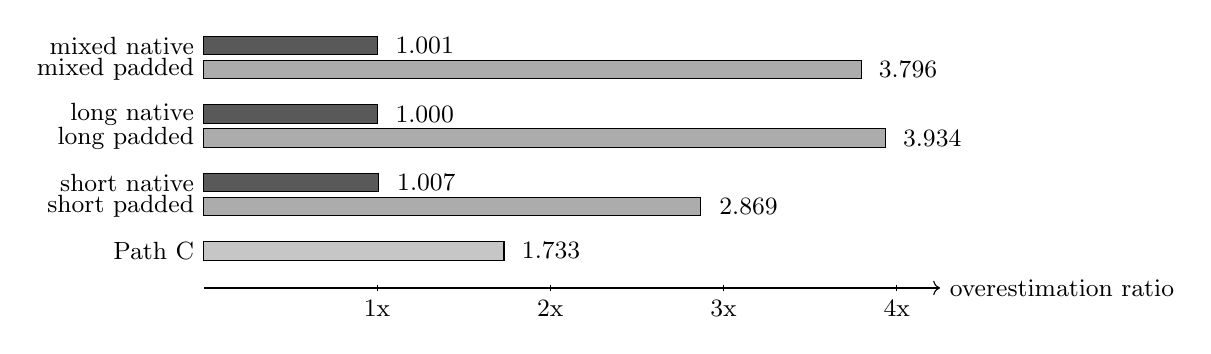
\begin{tikzpicture}[x=2.2cm,y=0.47cm,font=\small]
  \draw[->] (0,0) -- (4.25,0) node[right] {overestimation ratio};
  \foreach \x/\label in {1/1x,2/2x,3/3x,4/4x} {
    \draw (\x,0.08) -- (\x,-0.08) node[below] {\label};
  }
  \node[anchor=east] at (0,1) {Path C};
  \draw[fill=gray!45] (0,0.75) rectangle (1.733,1.25);
  \node[anchor=west] at (1.78,1) {1.733};

  \node[anchor=east] at (0,2.2) {short padded};
  \draw[fill=gray!65] (0,1.95) rectangle (2.869,2.45);
  \node[anchor=west] at (2.92,2.2) {2.869};
  \node[anchor=east] at (0,2.85) {short native};
  \draw[fill=black!65] (0,2.60) rectangle (1.007,3.10);
  \node[anchor=west] at (1.06,2.85) {1.007};

  \node[anchor=east] at (0,4.05) {long padded};
  \draw[fill=gray!65] (0,3.80) rectangle (3.934,4.30);
  \node[anchor=west] at (3.98,4.05) {3.934};
  \node[anchor=east] at (0,4.70) {long native};
  \draw[fill=black!65] (0,4.45) rectangle (1.000,4.95);
  \node[anchor=west] at (1.05,4.70) {1.000};

  \node[anchor=east] at (0,5.90) {mixed padded};
  \draw[fill=gray!65] (0,5.65) rectangle (3.796,6.15);
  \node[anchor=west] at (3.84,5.90) {3.796};
  \node[anchor=east] at (0,6.55) {mixed native};
  \draw[fill=black!65] (0,6.30) rectangle (1.001,6.80);
  \node[anchor=west] at (1.05,6.55) {1.001};
\end{tikzpicture}
\caption{Overestimation ratios in the observed \pathc{} matrix and the
deterministic RTX 3060 planner-only comparison. The native KV/state planner
model stays near useful bytes in the synthetic pack, while the padded model
reserves substantially more.}
\label{fig:ratios}
\end{figure*}

\textbf{Interpretation.}
Figure~\ref{fig:ratios} makes the planner distinction visible. In the synthetic
pack, the \plannernative{} model estimates close to useful bytes for all three
workloads. The \plannerpad{} model ranges from 2.868770x to 3.934376x. The
large workloads still have virtual OOM under both planner models because the
useful demand itself exceeds the target profile; this is a capacity result, not
a failure of the native accounting model.

\subsection{Evidence Boundary}

The two tracks support the same narrow claim: hybrid cache over-reservation is
visible in planner artifacts, and a native KV/state planner model can avoid
the padded planner's accounting overhead in deterministic planner replay. They
do not measure live serving memory, request admission, latency, throughput,
quality, or accuracy. They also do not establish controlled substitution
readiness, because the observed run does not resolve Mamba state-index and
state tensor contracts.

\section{Limitations}

The observed matrix covers one model, one vLLM version, two sequence lengths,
two memory-utilization settings, and \texttt{max\_num\_seqs=1}. The RTX 3060
pack is synthetic and planner-only. These limits are appropriate for a
diagnostic paper, but they bound the claims. A stronger systems paper would
need multi-model evidence, controlled mutation hooks, Mamba state contracts,
and live serving measurements.

\section{Conclusion}

Hybrid Attention/Mamba serving exposes an accounting problem before it exposes
an allocator replacement problem. \tool{} \pathc{} shows that planner-level
over-reservation can be diagnosed from committed vLLM planner artifacts without
changing runtime state. The workshop contribution is a clean diagnostic
workflow, a bounded vLLM planner matrix, and a deterministic planner-only
comparison that separates supported advisory evidence from future runtime
integration work.

\bibliographystyle{plain}
\bibliography{references}

\end{document}
